\begingroup
	\pgfdeclarelayer{background layer}
	\pgfsetlayers{background layer,main}
	\tikzstyle{zero}=[circle,draw=black,fill=white,inner sep=0pt,minimum size=2.5mm]
	\tikzstyle{one}=[circle,draw=black,fill=black,inner sep=0pt,minimum size=2.5mm]
	\tikzstyle{two}=[circle,draw=black,fill=gray,inner sep=0pt,minimum size=2.5mm]
		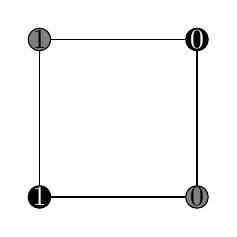
\begin{tikzpicture}
			\node [white] (a) at (1,1) [one] {$0$};
			\node (1) at (-1,1) [two] {$1$};
			\node [white] (b) at (-1,-1) [one] {$1$};
			\node (2) at (1,-1) [two] {$0$};
			
			\draw (1)--(b)--(2)--(a)--(1);		
		\end{tikzpicture}
	%\label{fig:eg_octahedral_1_sphere}	
\endgroup